\subsubsection{Embedding System and Router}
\label{sec:emb_sys_and_router}
The main result of this study was the creation of two key components: a flexible embedding
subsystem and a trainable router for the MoTE unit. These developments not only provide
a solid foundation for the further development of FinABYSS, but also open up a wide scope
for use in related application projects.

As part of the study, we conducted a series of experiments to select optimal combinations
of embedding models, DR methods, and clustering algorithms, using different
metrics to adjust hyperparameters. At the first stage, the basic chain consisted of ModernBERT,
UMAP (cosine metric), HDBSCAN (Euclidean metric) was optimized by the silhouette coefficient.
Despite the satisfactory results, we noted a strong dependence on the cluster structure and
the sensitivity of the silhouette to the shape of the clusters, which appeared to be arbitrary
shapes in our data.

The second stage repeated the same bundle, but the DBCV index was chosen as the target metric. Due
to the DBCV property of taking into account density features and heterogeneity of the point
distribution, hyperparameters selected for DBCV provided more semantically consistent and dense
clusters.

Finally, we tested base generally pre-trained and fine-tuned STS ("gte-modernbert-base")
versions of ModernBERT \parencite{Warner2024ModernBERT, MGTE2024}
in combination with UMAP, with cosine and $L_2$-Euclidean metric, and the same HDBSCAN,
also configured for euclidean and $L_2$-Euclidean distance (Table \ref{tab:experiment_configs}).
However, this combination was inferior to the previous one: the DBCV index was only 0.4032
against 0.4763 for the cosine + euclidean pair (Table \ref{tab:experiment_results}).

\begin{longtable}[c]{|l|ll|}
    \caption{Description of the final configurations of experiments conducted on a subsample of 10,000 embeddings.}
    \label{tab:experiment_configs}\\
    \hline
    \multicolumn{1}{|c|}{\multirow{2}{*}{\textbf{Model}}} & \multicolumn{2}{c|}{\textbf{Configuration}}                         \\ \cline{2-3}
    \multicolumn{1}{|c|}{}                                 & \multicolumn{1}{c|}{(I)}               & \multicolumn{1}{c|}{(II)}  \\ \hline
    \endfirsthead

    \endhead

    UMAP    & \multicolumn{1}{l|}{$L_2$-Euclidean} & \multicolumn{1}{l|}{Cosine}    \\
    HDBSCAN & \multicolumn{1}{l|}{$L_2$-Euclidean} & \multicolumn{1}{l|}{Euclidean} \\ \hline
\end{longtable}

Additional analysis of the noise points and cluster structure confirmed this advantage
(Table \ref{tab:experiment_results}). When using the $L_2$-Euclidean metric, the proportion
of noise points reached 42.16\%, and the number of clusters was 97 (with a maximum size
of 3,220 points and a minimum size of 260). For the cosine + euclidean pair, the noise was
only 36.18\%, and the number of clusters increased to 162; at the same time, the maximum
cluster increased to 3,742 points, and the minimum decreased to 109. Thus, the "cosine +
euclidean" approach demonstrated a better ratio of cluster density and separability.

% Please add the following required packages to your document preamble:
% \usepackage{multirow}
% \usepackage{longtable}
\begin{table}[!htbp]
\begin{longtable}[c]{|cl|cc|}
    \caption{Summary table of the results of hyperparameter optimization performed for three specified configurations on a subsample of 10,000 embeddings.}
    \label{tab:experiment_results}\\
    \hline
    \multicolumn{2}{|c|}{\multirow{2}{*}{\textbf{Best trial}}} & \multicolumn{2}{c|}{\textbf{Configuration}}                                                \\ \cline{3-4}
    \multicolumn{2}{|c|}{}                                     & \multicolumn{1}{c|}{(I)} & \multicolumn{1}{c|}{(II)} \\ \hline
    \endfirsthead

    \endhead

    \hline
    \endfoot

    \endlastfoot

    \multicolumn{1}{|c|}{\multirow{7}{*}{\textbf{Hyperparameters}}} & n\_components            & \multicolumn{1}{c|}{47}                & \multicolumn{1}{c|}{41}             \\
    \multicolumn{1}{|c|}{}                                          & n\_neighbors             & \multicolumn{1}{c|}{70}                & \multicolumn{1}{c|}{75}             \\
    \multicolumn{1}{|c|}{}                                          & min\_dist                & \multicolumn{1}{c|}{0,0}               & \multicolumn{1}{c|}{0,065}          \\
    \multicolumn{1}{|c|}{}                                          & spread                   & \multicolumn{1}{c|}{6,5}               & \multicolumn{1}{c|}{6,4}            \\
    \multicolumn{1}{|c|}{}                                          & negative\_sample\_rate   & \multicolumn{1}{c|}{10}                & \multicolumn{1}{c|}{11}             \\
    \multicolumn{1}{|c|}{}                                          & min\_cluster\_size       & \multicolumn{1}{c|}{360}               & \multicolumn{1}{c|}{145}            \\
    \multicolumn{1}{|c|}{}                                          & min\_samples             & \multicolumn{1}{c|}{180}               & \multicolumn{1}{c|}{170}            \\ \hline
    \multicolumn{1}{|c|}{\multirow{5}{*}{\textbf{Statistics}}}      & Max cluster size         & \multicolumn{1}{c|}{3824}              & \multicolumn{1}{c|}{2558}           \\
    \multicolumn{1}{|c|}{}                                          & Min cluster size         & \multicolumn{1}{c|}{365}               & \multicolumn{1}{c|}{147}            \\
    \multicolumn{1}{|c|}{}                                          & Total clusters           & \multicolumn{1}{c|}{73}                & \multicolumn{1}{c|}{141}            \\
    \multicolumn{1}{|c|}{}                                          & Noise \%                 & \multicolumn{1}{c|}{\textbf{39,54\%}}  & \multicolumn{1}{c|}{43,38\%}        \\
    \multicolumn{1}{|c|}{}                                          & DBCV Index               & \multicolumn{1}{c|}{0,397}             & \multicolumn{1}{c|}{\textbf{0,407}} \\ \hline
\end{longtable}
\end{table}

The experimental results clearly indicate the superiority of the ModernBERT + UMAP scheme with cosine
metric and HDBSCAN with Euclidean distance in the tasks of topical clustering of financial texts.
Combined with DBCV index optimization, this approach forms the most semantically coherent groups,
minimizes the proportion of noise instances, and provides a more stable basis for subsequent training
of the MoTE router.

Nevertheless, unfortunately, obvious problematic areas of the current implementation have also been
identified. The resulting clusters and their structure cannot be incrementally updated with streaming
new publications, which happens for several reasons. Firstly, the trained model is a GPU implementation
from the cuML library, in which critical errors were discovered in the code version 25.02
\parencite{cuml2020machine} only after conducting research. Secondly, the chosen UMAP algorithm
does not work well enough in incremental mode by its nature, which is why there are other implementations,
such as AlignedUMAP \parencite{mcinnes2018umap-software} or ParametricUMAP based on a neural network
as a basic model \parencite{ParametricUMAP2020}. Unfortunately, both of these implementations are available
exclusively for training on a central rather than a GPU. And there are not enough computing resources
for learning on a central processor in the context of the current study.

Thus, the bottleneck of this study and the proposed solution is the lack of computing power for training
models, which will be improved in further research.

\subsubsection{Semantic Map}

Finally, based on the developed embedding subsystem and the MoTE router, a separate UMAP model was trained,
designed to translate vectors from the intermediate latent clustering space into a two-dimensional
representation convenient for visual analysis. It is this projection that underlies the Semantic Map
of Financial Publications, one of the key components of the FinABYSS interface, which provides a deep
and intuitive study of the thematic structure of news streams.

\begin{figure}[H]
    \centering
    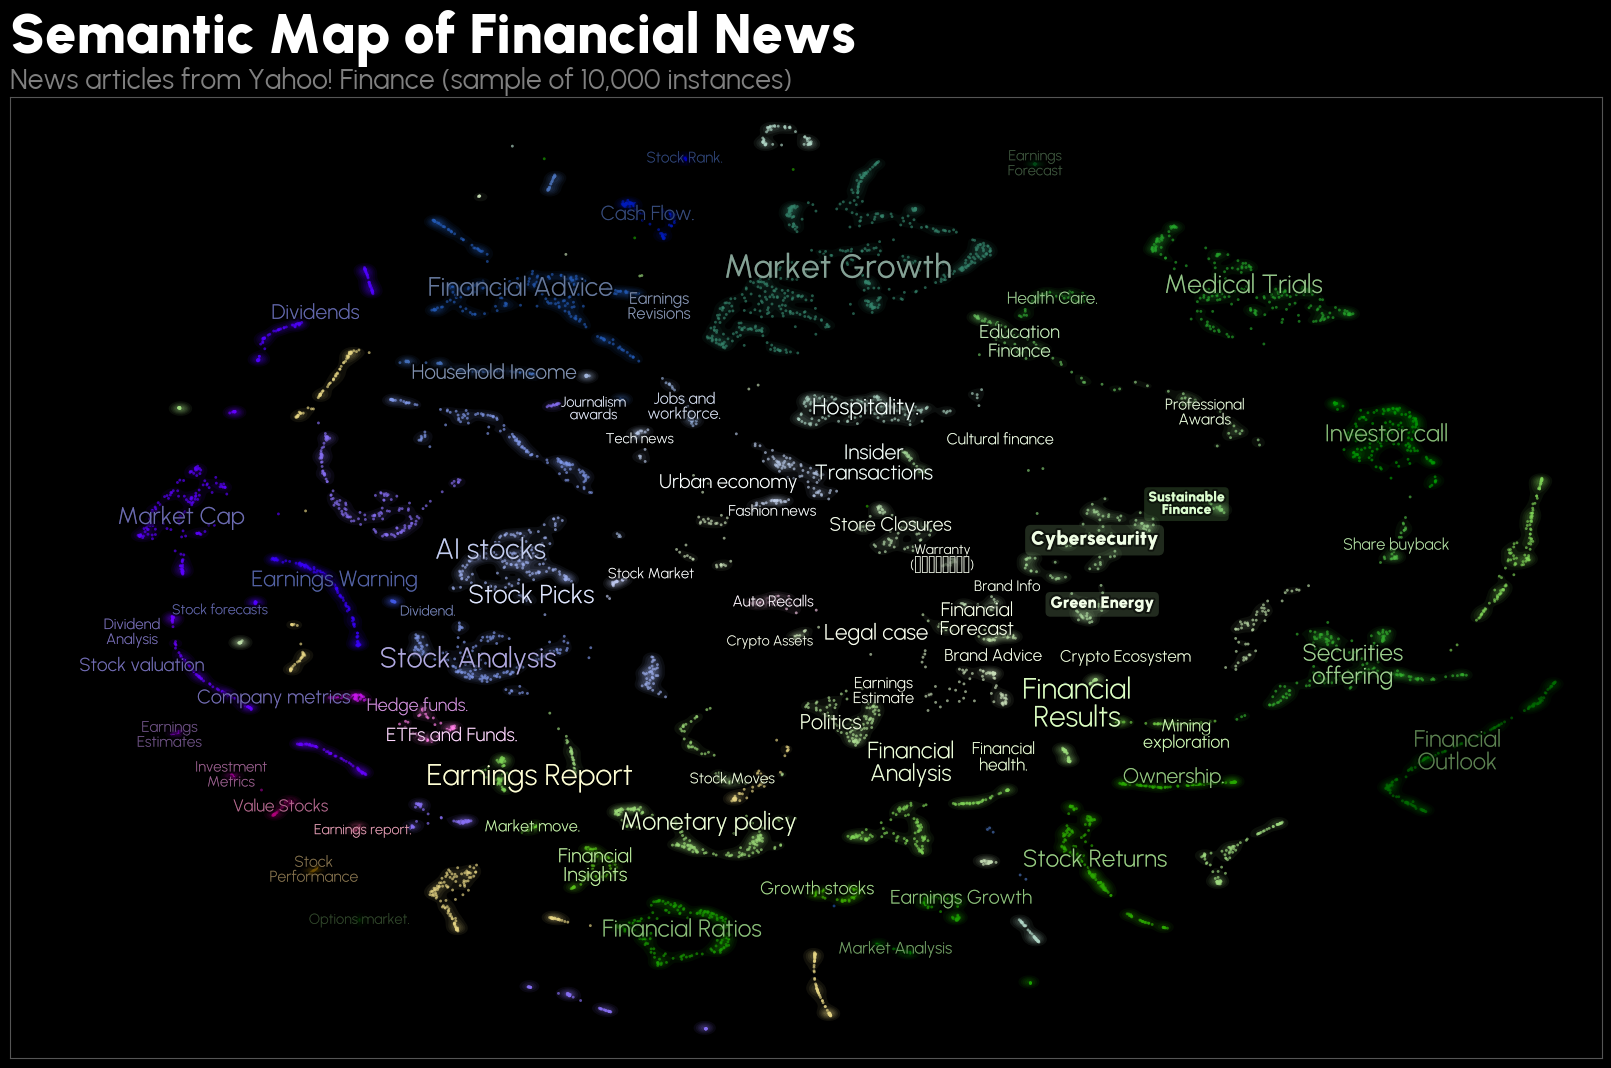
\includegraphics[width=1\linewidth]{img/semantic_map.png}
    \caption{Semantic map (demo version) of a sample of 10,000 financial publications
    from September 17, 2023 to March 18, 2025, clustered by financial topics.}
    \label{fig:semantic_map}
\end{figure}

First, a static version of the map was implemented, which displays 100,000 financial items from September 2023
to March 2025, divided into clusters by subject (Figure \ref{fig:semantic_map}). Each cluster is marked
with an automatically generated tag word without any manual annotation. Despite the automatic nature
of the assignment, the labels turned out to be representative: dense groups of articles on healthcare,
"Sustainable Finance," "Cybersecurity," and "Green Energy" are located side by side, reflecting their semantic
proximity. The same thing happens with the "Politics" and "Monetary Policy" clusters.

However, the static map only demonstrates the potential of UMAP projection. The FinABYSS interactive Semantic
map goes far beyond the simple visualization of points:

\begin{itemize}
    \item Hovering over any point reveals the metadata of the article: title, date and time of publication,
    hierarchical topic (macro/meso/microtheme), author and source. At the same time, a preview of the full
    text and a direct link to the original publication are available.
    \item The keyword search engine allows you to quickly filter articles containing special terms. The search
    can be combined with filters by date range, publication volume, and other numerical attributes (for example,
    text volume or number of views), which makes it easier to spot historical events and triggers on the graph.
    \item The Sources and Topics section makes it possible to include and exclude news sources or target clusters,
    helping to focus on relevant publications in complex analytical scenarios.
    \item A word cloud function is also available for articles, which is formed based on the most frequent words
    found in a selected group of texts. The word cloud instantly displays the dominant terms and discussion patterns,
    which complements the quantitative outline of the graph with qualitative characteristics.
\end{itemize}

Thus, the FinABYSS semantic map is a full-fledged analytical system that combines the power of the selected UMAP
and HDBSCAN models, and with further development, the hybrid CNN-LSTM architecture and the MoE approach to sentiment
analysis. It provides the researcher with the opportunity not only to visually distinguish named clusters and
their mutual arrangement, but also to delve deeply into the content of each publication, combining automatic and
manual analysis methods.

The developed interactive Semantic map is a natural continuation of the previous FinABYSS modules. All the pipeline
links are connected in a single chain. The tool offers the user a transparent, scalable and flexibly customizable
interface for semantic research of financial news, where each element --- from cluster labels to a cloud
of words --- reflects the results of the computational logic of the system and supports expert solutions
in the analysis of market processes.

\subsubsection{Dynamic Topic Modeling}

In addition to the Semantic Map, FinABYSS provides powerful tools for analyzing the linguistic features
of formed thematic groups and dynamic temporal modeling of topics. All incoming texts go through
the post-processing pipeline described in \hyperref[sec:sys_dev]{Section 2.4} in the context of the Analytical GUI
(see \hyperref[sec:gui]{Section 3.1.6}), where each document is assigned a prevailing theme, and
then the corresponding lexical features are extracted and aggregated.

Thus, the system visualizes the frequency distribution of the most relevant words within the selected topic
(Figure \ref{fig:topics_words_freqs}). This linguistic panel serves two purposes:

\begin{itemize}
    \item Firstly, after developing the system, it allows to validate the quality of the generated topics
    and assess how unique and semantically homogeneous they are, in manual mode.
    \item Secondly, this functionality can be very useful when a financial analyst is first introduced
    to the system. A financial analyst working with FinABYSS for the first time gets an instant understanding
    of the content of each topic without deep reading of texts.
\end{itemize}

It was the latter fact that led to the inclusion of this functionality in the set of basic analytical GUI toolkit.

\begin{figure}[H]
    \centering
    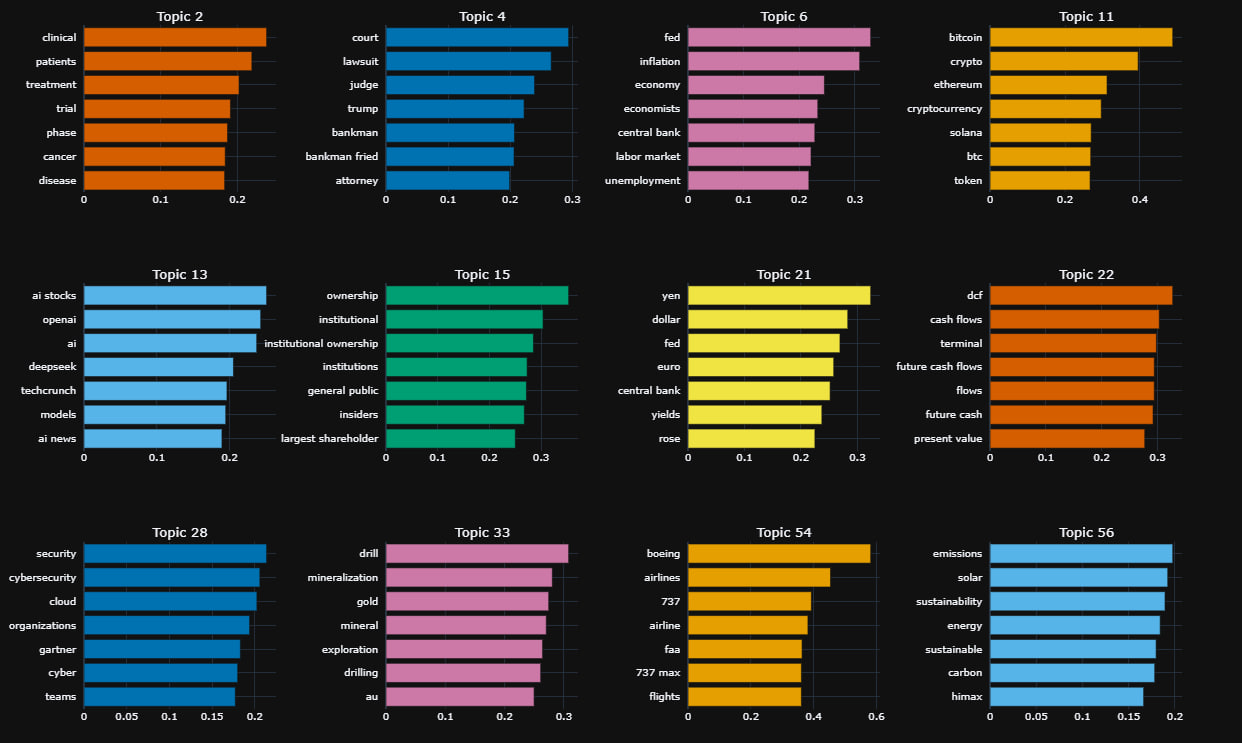
\includegraphics[width=1\linewidth]{img/topics_words_freqs.png}
    \caption{Terms ranked by relevance for a sample of 12 topics.}
    \label{fig:topics_words_freqs}
\end{figure}

To illustrate this functionality, a subsample of 100,000 publications was randomly generated and 12 topics
were selected within them for display. Among the sample, all topics undoubtedly have practical significance
for financial markets. Moreover, there are more general industry topics such as:

\begin{itemize}
    \item Topic 2 related to the pharmaceutical industry;
    \item Topic 13 related to the artificial intelligence sector;
    \item Topic 28 related to cybersecurity;
    \item Topic 33 related to the mining industry;
    \item Topic 54, related to the aviation industry.
\end{itemize}

On the other hand, the sample also includes a common topic that is on the agenda in finance --- Topic 56,
which clearly relates to ESG. Finally, there are highly specialized financial topics that were also identified
automatically:

\begin{itemize}
    \item Topic 4 related to lawsuits and proceedings, which is potentially extremely important and
    influential in the context of asset pricing;
    \item Topic 6 related to external economic factors and the economy in general;
    \item Topic 11, directly related to the asset market, namely cryptocurrencies;
    \item Topic 15 related to company ownership rights;
    \item Topic 21 related to the foreign exchange market;
    \item Topic 22 related to cash flows, including future, present and discounted
    cash flows.
\end{itemize}

So, we can observe the linguistic features of the topics, as well as very quickly and effectively study
both the differences between them and specific topics in depth.

On the other hand, it would be extremely useful to understand how topics change over time, because the information
media space is extremely unstable, and the agenda in modern society is changing extremely quickly. Thus, FinABYSS
implements dynamic thematic modeling through an interactive graph of topical time series.

\begin{figure}[H]
    \centering
    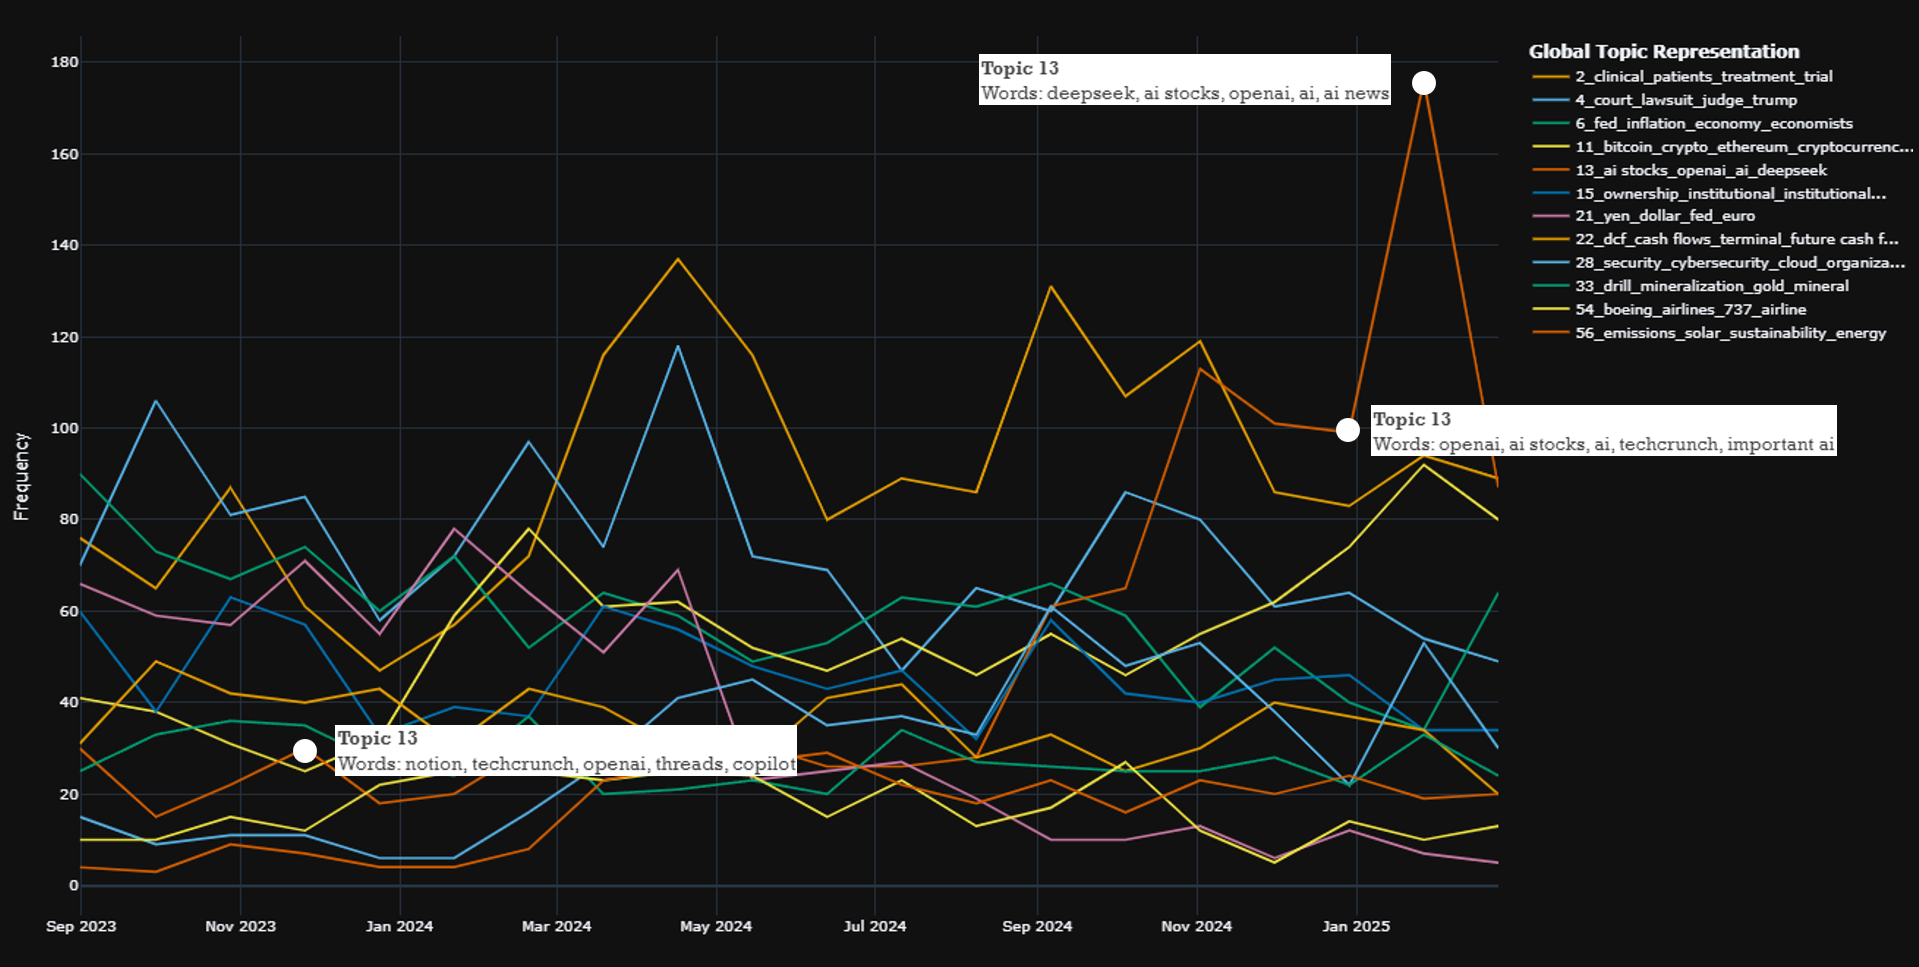
\includegraphics[width=1\linewidth]{img/dynamic_topic_modeling.png}
    \caption{Evolutionary dynamic topic modeling of the most relevant terms
    for a sample of 12 topics for the period from September 17, 2023
    to March 18, 2025.}
    \label{fig:dtm}
\end{figure}

The Figure \ref{fig:dtm} shows the same subsample of 12 topics. The abscissa axis reflects the publication
interval (configurable: from daily to monthly or annual), the ordinate axis is the number of articles on each
topic for the corresponding period. When hovering over the cursor, the five most representative words describing
the topic in this time window are displayed. The user can change the number of words displayed.

The advantages of this approach are obvious:

\begin{itemize}
    \item Early detection of trends. The analyst can observe the appearance of new lexical markers or the growth
    of publication activity in thematic groups, which serves as a signal of emerging events.
    \item Tracking cyclical phenomena. So, for Topic 13 (AI), the word TechCrunch appears on the chart in December
    2023 and December 2024, the name of one of the largest and most prestigious conferences in the fields of IT and AI.
    Every year, the conference produces many of the largest startups, which later receive large amounts of funding.
    Thus, with this visualization, the analyst can keep up to date with cyclical events that are significant for finance
    with less effort.
    \item Reaction to force majeure events. In February 2025, there is a sharp peak on the same Topic 13 due
    to the announcement of the Chinese LLM DeepSeek R1. This incident is extremely important, as it subsequently
    caused the collapse of Nvidia shares, the largest company supplying computing equipment.
\end{itemize}

Thus, FinABYSS is not limited to the static construction of thematic clusters: interaction with linguistic metrics
and temporal trends turns the system into a universal platform for financial analytics. The expert can switch from
macro-trends to micro-lexical details in a few clicks, combine filters by date, source and subject, study the evolution
of terminology and quickly respond to the appearance of new keywords or abnormal frequency changes. This makes FinABYSS
not just a clustering tool, but a full-fledged ecosystem for semantic monitoring and forecasting the impact of media
signals on the dynamics of financial assets.

\subsubsection{Practical Importance}
\label{sec:practical_importance}

To summarize, it is worth emphasizing that the FinABYSS system is not just a set of models, but a full-fledged
tool for rapid detection of critical signals in financial markets. Semantic map, deep topical clustering
and news time series allow financial analysts to instantly react to unexpected events, reduce risks
and profit.

Thus, looking solely at the functionality of the Semantic Map, one can find several critical events that were
immediately reflected in the “Legal case” thematic cluster in a timely manner after they hit the web.

The first illustrative example (Figure \ref{fig:citi_group}) demonstrates how an article dated May 22, 2024
affected the stock price of the target company. This news highlighted the scandal of the collapse of the value
of European stocks due to insufficient control over trading operations by one of the 4 largest banks
in the world --- Citi Group (C.NYSE) --- whose shares are traded on the New York Stock Exchange. After this news,
which also announced the imposition of a record fine on the bank by the British government, the company's shares
fell almost 4\% over the next 28 hours. Over the next 23 days, as litigation, additional reports and delayed
market reaction took place, the price fell nearly 10\%.

\begin{figure}[H]
    \centering
    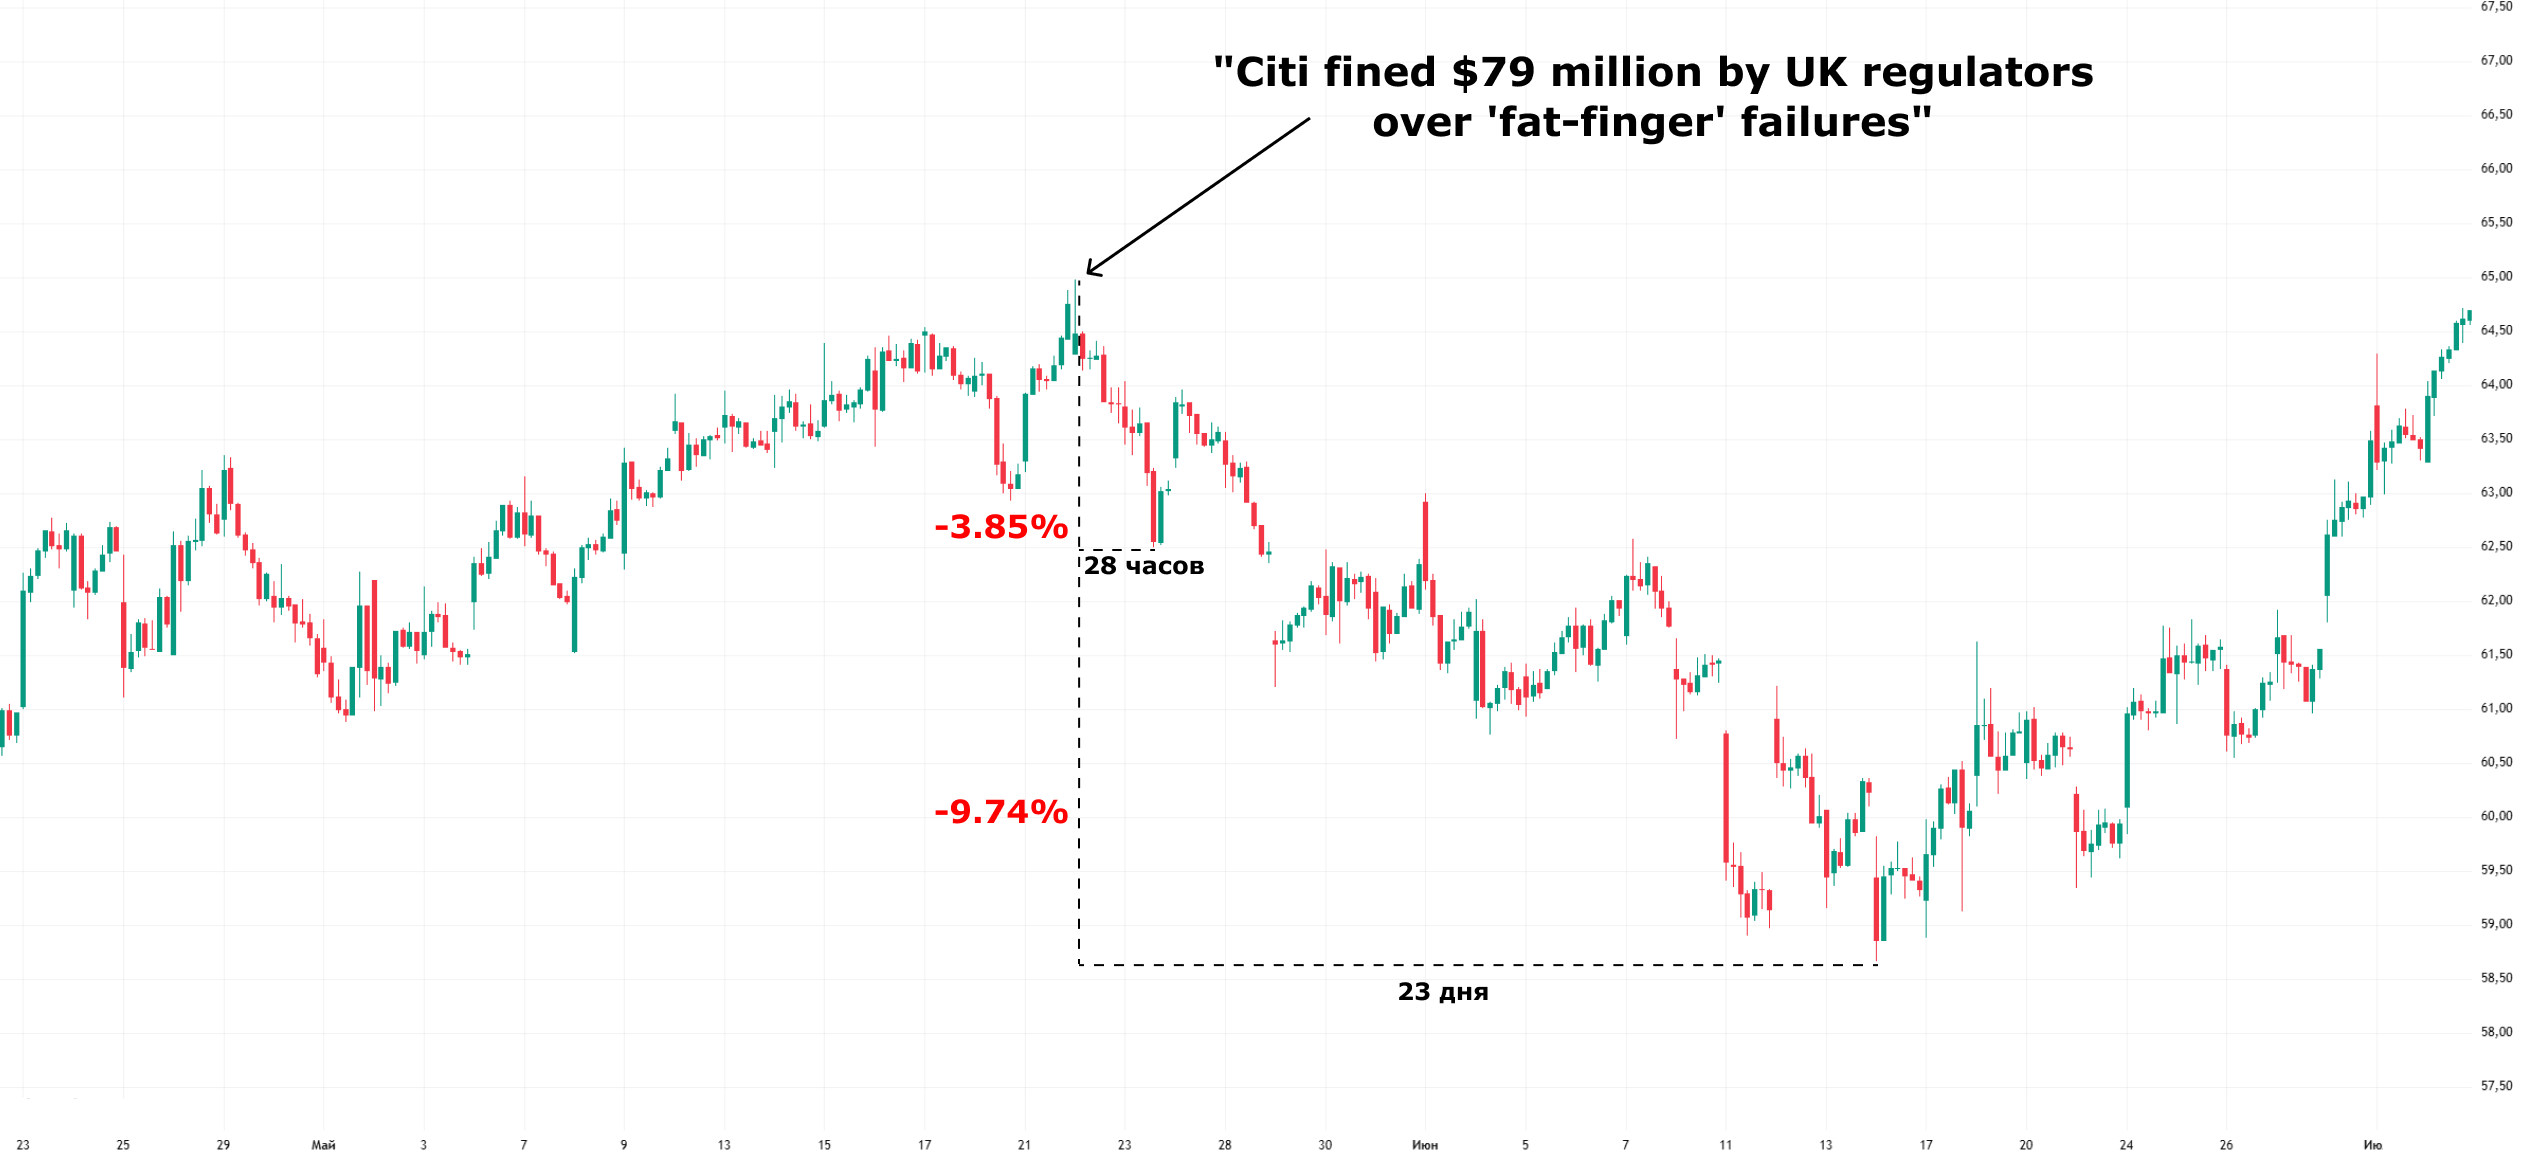
\includegraphics[width=1\linewidth]{img/citi_group.png}
    \caption{An example of the fall in the share price of one of the largest US banks, Citi Group
    (C.NYSE), due to allegations of insufficient control over trading operations, which caused
    a fall in European shares}
    \label{fig:citi_group}
\end{figure}

The Reuters news article itself signaled a sell signal, while the Figure \ref{fig:citi_group} clearly shows
a tipping point with a sharp drop in price, a small pullback and a further change in the global trend for almost
a month.

Without FinABYSS, such signals are often lost in the news flow, while the developed system simplifies the detection
of trigger events by implementing the ability to track clusters significant for a particular portfolio.

The second case study relates to a news item dated August 30, 2024 about a possible license revocation and AU\$67
million fine against Australia's largest gambling company, The Star Entertainment Group LTD
(Figure \ref{fig:star_entertainment}). News reported allegations of money laundering. The shares were frozen
for a month, and when trading resumed, their value collapsed by 55\%.

\begin{figure}[H]
    \centering
    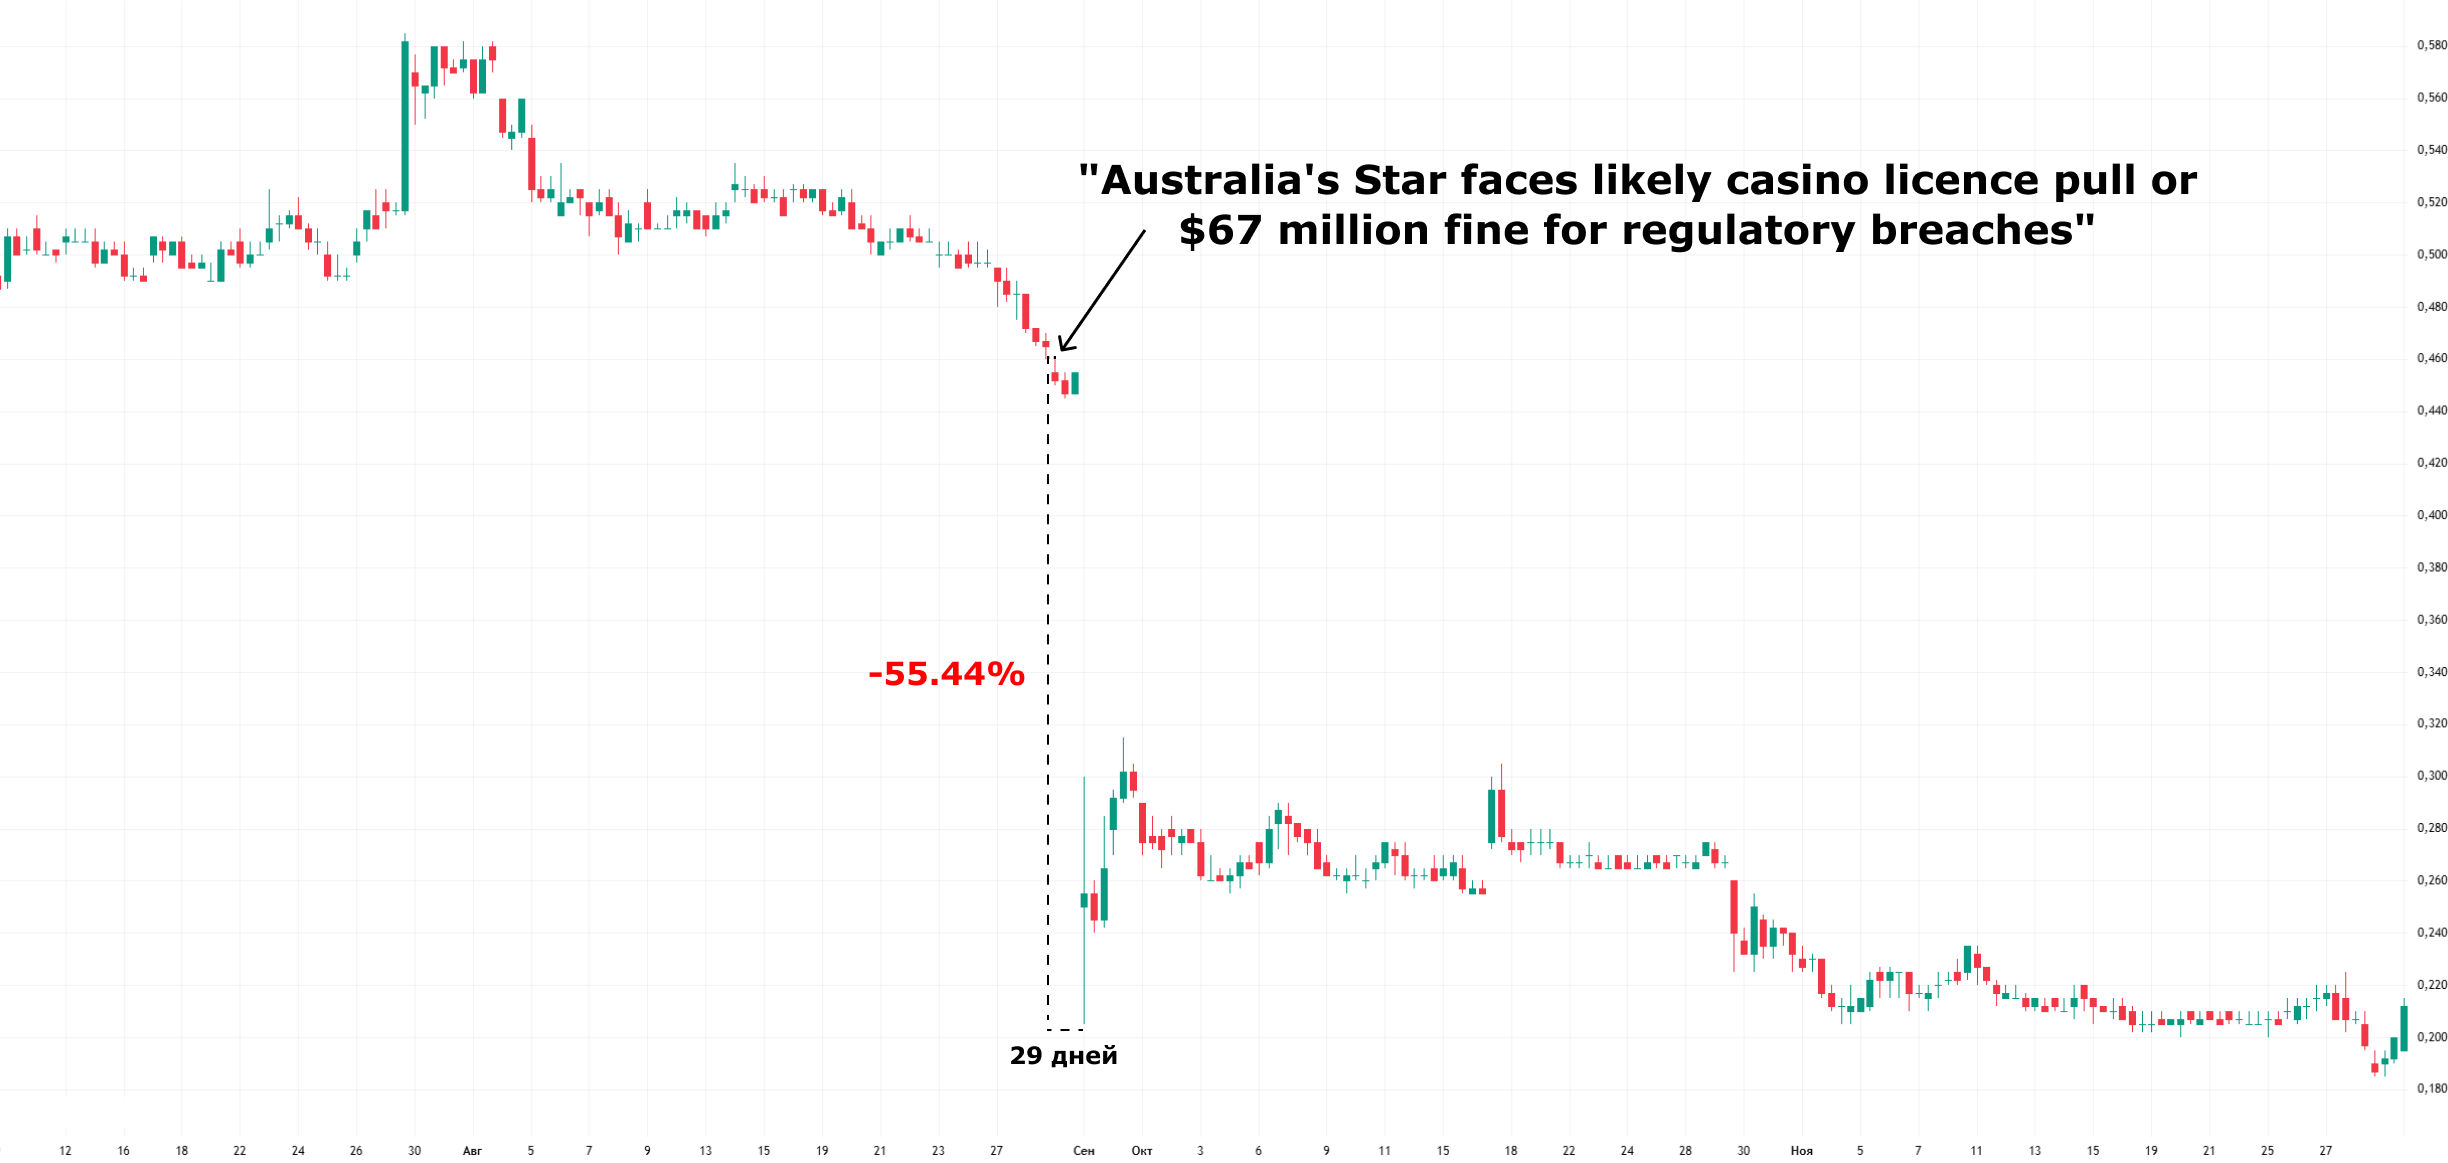
\includegraphics[width=1\linewidth]{img/star_entertainment.png}
    \caption{An example of Australian company The Star Entertainment Group LTD (SGR.ASX) shares
    collapsing and being temporarily halted from trading due to money laundering litigation.}
    \label{fig:star_entertainment}
\end{figure}

It is important to note that trading was halted 24 hours after the news was published, which is a sufficient
interval for a sell signal to be detected. However, for the average investor not involved in intraday trading,
this signal would very likely have been undetectable, leading to the dire situation of an investor unable to sell
a depreciating asset and forced to hold an obvious loss indefinitely.

In both cases, with FinABYSS, a financial analyst or investor would be among the first to recognize these incidents
and react immediately to market signals. The simplest way to learn about triggers in a timely manner is the asset-based
tracking module, which allows you to set filters by specific ticker, source, and topic to receive only targeted signals.

Eventually, once the architecture proposed in \hyperref[sec:architecture]{Section 3.1} is fully implemented and trained, it will be possible
to customize the filtering of news by its sentiment, as well as setting a custom threshold to detect meaningfully
positive or negative news.

FinABYSS thus takes financial analytics to a whole new level: instead of haphazard monitoring of media and articles,
it gets ready-to-action alerts, visualization, and predictive support. The semantic map is already becoming an integral
part of the workflow, and its value will only grow with the expansion of modalities and the introduction of a predictive
mechanism.